\chapter{Conclusion}
\section{Future Work}

\subsection{Fill the gaps}
SecureWilly's development has been completed so that its goal is achieved but certainly, there are still several features to be fixed. Some of them could be the following:
\begin{itemize}
\item Extract more rules in static analysis
\item Include other syntax forms of Dockerfile instructions and Docker Compose options to static\_parser.py
\item More rules to prevent attacks
\item More flexible User Interface
\item Support interactive test plans of the project, not only script commands
\item Change python scripts into executables (maybe write programs in Go) so that python interpreter is not a requirement
\item Fix the conflict of multiple containers using the same image, when a docker-compose file is not provided
\item Fix clearing volumes by detecting docker project's volumes and deleting them, instead of using docker volume prune
\end{itemize}
SecureWilly is an open source project and contributions are more than welcome. You can find it on GitHub: \url{https://github.com/FaniD/SecureWilly}

\subsection{AppArmor}
\subsubsection{AppArmor 3.0 and future features}
AppArmor 3.0 is coming and is bringing several new shiny features with it. \cite{app3seth}

First of all, since AppArmor is the main tool SecureWilly is using, we are happy to hear that AppArmor 3.0 will compile and execute its policies much faster. AppArmor policies are compiled from the text to an optimized state machine that can be executed quickly in the kernel. The state machines are cached to speed up future boots. Current version of AppArmor uses a single binary policy cache. This causes several underlying risks. For example, if the default location /etc/apparmor.d/cache is moved or there is a change in kernel, the single cache has to be rebuilt on boot. Situations like that slows down the boot.
  
The upcoming AppArmor version will have multiple caches based on hashing the ABI exposed by the running kernel. In the end, swapping between kernels should be much faster.

Furthermore, AppArmor is working on mediating access to coarse-grained networking, dbus and unix sockets. We should adapt new rules in SecureWilly as soon as the implementations are completed, to improve isolation referring to network, dbus and unix sockets. 

It is also in AppArmor's plans to allow users to supply their own profiles and even restrict policies for specific users and groups. This will open up namespaces to user defined policy and it may help adapt user namespaces to SecureWilly's profiles by creating policies on container's user namespaces. Of course, this will expose more kernel interfaces to userspace, so it should be used thoughtfully.

AppArmor has already had the ability to confine users or do roles for quite a while. 
An AppArmor profile applies to an executable program; if a portion of the program needs different access permissions than other portions need, the program can change hats via change\_hat to a different role, also known as a subprofile. The pam\_apparmor PAM module allows applications to confine authenticated users into subprofiles based on group names, user names, or a default profile. To accomplish this, pam\_apparmor needs to be registered as a PAM session module. \cite{susepam}
Pam\_apparmor creates mappings through policy using hats and requires task calling into pam to be confined. Roles use policy inheritance, which means that a task which is confined by a profile, demands all its children to be confined by the same profile.

However, it is a fact that pam\_apparmor is a difficult tool to setup and has several limitations. In order to work properly, pam\_apparmor needs the whole system to be confined. This causes plenty of issues since total system confinement is not what most people want and not what most policy is setup for. These issues have led pam\_apparmor to being rather unpopular and SecureWilly hasn't adapted it either for the same reasons.

AppArmor is willing to work on it in the future and upgrade pam\_apparmor. It's going to have a config file, it's going to be using change\_profile instead of change\_hat, a user condition is going to include in policies and last but not least it will not require total system confinement. All in all, pam\_apparmor is going to get far easier to use than it is now and SecureWilly is open to reconsider and adapt this tool.

Other possible directions for the future that AppArmor is considering of following and that may help us in container isolation are cgroups and chroot (more than capability SYS\_CHROOT which is currently the only way to allow syscall chroot). Cgroups would be very helpful for restricting access to resources on containers and thus achieving hardware isolation on containers. Chroot implementations would be of great help if we use them in SecureWilly's profiles to restrict the chroot syscall as if it stays within a container and not allow it to happen out of the container and help attackers chroot to host or other containers.

\subsubsection{Policy Namespaces and Stacking}
Two other recent developments of AppArmor that should be attached to SecureWilly are policy namespaces and policy stacking. \cite{app3suse}
\begin{description}
\item[Policy namespaces:] AppArmor has multiple namespaces for policies. Docker can own its profiles and other host's applications can own their profiles. Policy namespaces are hierarchical.  Each namespace has its own set of profiles and its own unconfined state. A policy namespace defines a view, where a parent can see policies in its children and below and through this view we can answer questions like where can a policy be loaded, who can load a policy to where etc. 

\item[Policy stacking:] AppArmor policies can be stacked. Host could be protected from containers with one set of profiles, and then the container could use AppArmor profiles itself to keep its services and users separated from the host and do whatever they need to do. For example, blanket profiles can be applied to all users in a group to keep them in a certain portion of a system, such as “no net” profile or “no capabilities” profile that could be stacked with other profiles and have a very creative policy with all these profiles combined. SecureWilly should use this feature for multiservices projects, to keep a global stacked policy for all services in order to protect the host as well as separate profiles for each service in alignment with what each service requests to do.
\end{description}

If we combine policy namespaces and policy stacking then we have an interesting result.

\begin{figure}[h!]
  \centering
   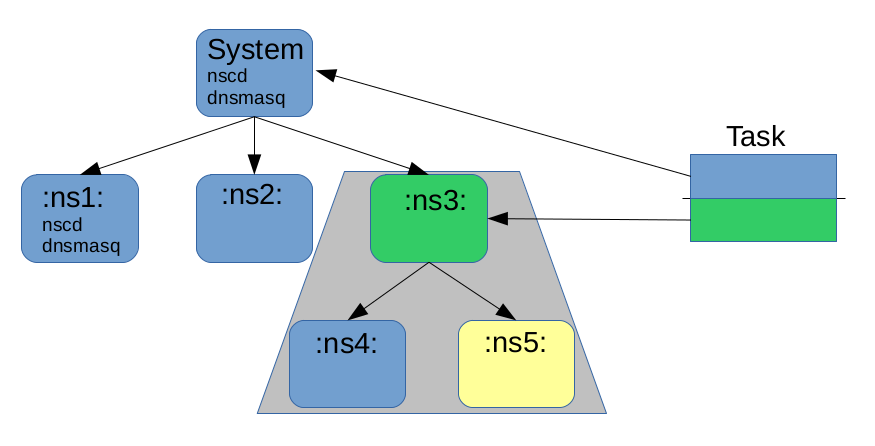
\includegraphics[width=0.9\linewidth]{./figures/policystacking1.png}
   \caption{AppArmor Policy Stacking}
\end{figure}

Let's examine the figure 6.1. In this tree, we have a system with some hierarchical policy namespaces and a task which is confined by a stacked policy including profiles from system and ns3. What makes the combination of these two interesting, is that although the task is confined by both profiles, it can only see policy from ns3 and below. This is exactly what we are seeking for docker containers. We want containers to be restricted by host for outer namespaces and allowed to load extra policy to restrict themselves in inner namespaces without knowing the existence of the outer namespace.
This could have a further extent to policies for nesting containers within containers.
\hfil\break\hfil\break

To sum up, as soon as AppArmor brings new features SecureWilly is ready to investigate them and adapt them in order to defend container's isolation.

\subsection{Confront other types of attacks}
Currently, SecureWilly focuses on preventing container breakout attacks. Research could be made in other types of attacks in order to create rules that would prevent more isolation violations. There are certainly many aspects that we could examine in order to break down into pieces other types of attacks, like we did with container breakout and through this procedure we may come up with a set of rules that could possibly block some instances of these attacks.

Specifically, DoS attacks could be prevented, if AppArmor had rules that involve cgroups. As we mentioned in the previous section, isolating cgroups in the future is an aspect that AppArmor is considering of. This means that as AppArmor gets more powerful, more attacks could be prevented by SecureWilly.

\subsection{SELinux}
SecureWilly is using AppArmor profiles but it could include SELinux and give user the choice between AppArmor or SELinux profile.

\subsection{Container orchestration}
SecureWilly already supports multi-service projects and succeeds in exporting a profile for each service. It is a fact though that there are several new aspects we can work with on this field.

This can be expanded and examine new horizons where SecureWilly will be used to support container orchestration platforms like Docker Swarm, Kubernetes, Apache Mesos, Cloud Foundry etc 

